\documentclass{article}[a4paper]

\usepackage[fleqn]{amsmath} % This package with the fleqn option aligns equations to the left
\setlength{\mathindent}{0pt} % Set indentation from the left margin

\usepackage{amssymb} % Required for math symbols
\usepackage{graphicx} % Required for inserting images
\usepackage{geometry}

\usepackage{float} % Use this package to control float behavior

\usepackage{algorithm}
\usepackage{algpseudocode}

\usepackage[backend=biber, style=authoryear, citestyle=authoryear]{biblatex}
\addbibresource{references.bib}

\geometry{a4paper, margin=1in}

{
\title{
    
\includegraphics[width=0.34\textwidth]{/Users/mlnick/documents/images/tsukuba-logo.png} \\
    \vspace{2mm}
    \textbf{Numerical Simulation} \\
    \vspace{3mm}    
    Project 3 \\
    Finite Difference Time Domain with Dynamic Current
}

\author{Mamanchuk Mykola, SID.202420671}
% \date{\today}
\date{\today}
}

\usepackage{listings}
\usepackage{color}

\definecolor{codegreen}{rgb}{0,0.6,0}
\definecolor{codegray}{rgb}{0.5,0.5,0.5}
\definecolor{codepurple}{rgb}{0.58,0,0.82}
\definecolor{backcolour}{rgb}{0.99,0.99,0.99}

\lstdefinestyle{mystyle}{
    backgroundcolor=\color{backcolour},   
    commentstyle=\color{codegreen},
    keywordstyle=\color{magenta},
    numberstyle=\tiny\color{codegray},
    stringstyle=\color{codepurple},
    basicstyle=\ttfamily\footnotesize,
    breakatwhitespace=false,         
    breaklines=true,                 
    captionpos=b,                    
    keepspaces=true,                 
    numbers=left,                    
    numbersep=5pt,                  
    showspaces=false,                
    showstringspaces=false,
    showtabs=false,                  
    tabsize=2
}
\lstset{style=mystyle}

\begin{document}

\maketitle

\section{Introduction}

This project aims to extend the capabilities of the Finite Difference Time Domain (FDTD) simulation by introducing a dynamic component of current, \( J \), arising from the motion of an ion and an electron. This addition is aimed at exploring how localized sources of current affect the electromagnetic fields within a simulation domain, providing insights into the interaction between electromagnetic waves and moving charges.

\section{Theory Related Essentials}

\subsection{Maxwell's Equations and FDTD}

The FDTD method is utilized for solving Maxwell's equations discretely in both space and time. This numerical method leverages Yee's algorithm to alternate between updating electric and magnetic fields, which ensures numerical stability and adherence to physical laws.

\subsubsection{Modified Maxwell's Equations}

Incorporating the motion of charged particles, the Maxwell's equations are modified to include the effects of currents generated by the particles. The equations for this project, accounting for the current generated by an ion and an electron at the simulation's center, are specified as:

\begin{itemize}
    \item \textbf{Electric Field Update:}
    \[
    E_y(i, n + 1) = E_y(i, n) + \frac{\Delta t}{\Delta x} \left[ B_z(i + 1/2, n + 1/2) - B_z(i - 1/2, n + 1/2) \right] - J_x(i, n)\Delta t
    \]
    where \( J_x(i, n) \) represents the current density at position \( i \) and time step \( n \), calculated based on the velocity and charge of the ion and electron.
    
    \item \textbf{Magnetic Field Update:}
    \[
    B_z(i + 1/2, n + 1/2) = B_z(i + 1/2, n - 1/2) - \frac{\Delta t}{\Delta x} \left[ E_y(i + 1, n) - E_y(i, n) \right]
    \]
\end{itemize}

These modified equations ensure that the electric field is influenced directly by the current, while the magnetic field is influenced indirectly through the electric field changes. This project investigates how these modifications impact the propagation and dynamics of electromagnetic fields in scenarios that mimic real-world physical phenomena.

In the subsequent sections, the implementation of these theoretical principles in the FDTD framework will be detailed, followed by a discussion and visualization of the results, illustrating the practical implications of integrating currents in electromagnetic field simulations.

\begin{itemize}
  \item \textbf{Electric Field Update:}
  \[
  \frac{\partial E_y}{\partial t} = \frac{1}{\epsilon_0} \left( \frac{\partial B_z}{\partial x} - J_x \right)
  \]
  Here, \(E_y\) is the y-component of the electric field, \(B_z\) is the z-component of the magnetic field, and \(J_x\) is the current density along x. This equation integrates the effect of both the magnetic field change and the electric current on the electric field evolution.

  \item \textbf{Magnetic Field Update:}
  \[
  \frac{\partial B_z}{\partial t} = -\mu_0 \frac{\partial E_y}{\partial x}
  \]
  This equation describes how the magnetic field evolves in response to the spatial variation of the electric field.
\end{itemize}

\section{Implementation and Initialization Details}

\subsection{Pseudocode}

Below you can see the pseudocode realization for the task.

\begin{algorithm}[H]
    \caption{1D FDTD Simulation with Current}
    \begin{algorithmic}[1]
    \State \textbf{Initialize} grid size $L$, time step $dt$, space step $dx$, and total time steps $T$
    \State \textbf{Initialize} arrays $Ey$, $Bz$, and $J$ with zeros
    \State \textbf{Set initial conditions}:
    \State $Ey[\frac{L}{2}] \gets 1$ \Comment{Initial impulse in the electric field}
    \State $J[\frac{L}{2}] \gets 1$ \Comment{Current density due to particle motion at center}
    \For{$t = 0$ to $T-1$}
        \State \textbf{Update magnetic field $Bz$}:
        \For{$i = 0$ to $L-2$}
            \State $Bz[i] \gets Bz[i] - \frac{dt}{dx} \cdot (Ey[i+1] - Ey[i])$
        \EndFor
        \State $Bz[L-1] \gets Bz[L-1] - \frac{dt}{dx} \cdot (Ey[0] - Ey[L-1])$ \Comment{Periodic boundary for $Bz$}
        \State \textbf{Update electric field $Ey$}:
        \For{$i = 1$ to $L-1$}
            \State $Ey[i] \gets Ey[i] - \frac{dt}{dx} \cdot (Bz[i] - Bz[i-1]) + J[i] \cdot dt$
        \EndFor
        \State $Ey[0] \gets Ey[0] - \frac{dt}{dx} \cdot (Bz[0] - Bz[L-1]) + J[0] \cdot dt$ \Comment{Periodic boundary for $Ey$}
    \EndFor
    \end{algorithmic}
\end{algorithm}

\subsection{Explanation of the Simulation Steps}

The pseudocode above outlines a 1D Finite Difference Time Domain (FDTD) simulation which incorporates both electric and magnetic fields, as well as a current density component. Here's a detailed breakdown of each step and the reasoning behind it:

\begin{enumerate}
    \item \textbf{Initialization:} The simulation space (grid) is defined with a specified number of points ($L$), and the temporal ($dt$) and spatial ($dx$) resolutions are set. Arrays for the electric field ($Ey$), magnetic field ($Bz$), and current density ($J$) are initialized to zero. This sets up a neutral field environment before introducing any electromagnetic disturbances.

    \item \textbf{Initial Conditions:} An initial impulse is introduced in the electric field at the center of the grid to mimic an instantaneous electromagnetic disturbance. Simultaneously, a current density is set at the same location to simulate the presence of moving charges (an ion and an electron). This setup is critical as it initiates the electromagnetic phenomena that the FDTD method will propagate through the simulation space.

    \item \textbf{Magnetic Field Update:} The magnetic field is updated using a finite difference approximation of Faraday's law of induction. This update step calculates the change in the magnetic field based on the spatial variation of the electric field. The subtraction of electric field values across adjacent points, scaled by the ratio of the time step to the space step, ensures that the simulation adheres to the Courant-Friedrichs-Lewy (CFL) condition for stability.

    \item \textbf{Periodic Boundary Conditions:} To simulate an effectively infinite or cyclic space, periodic boundary conditions are applied. This means the field values at the ends of the array affect each other, simulating a continuous looped space. This is essential for studying wave propagation in a bounded yet unbounded seeming medium.

    \item \textbf{Electric Field Update:} Similar to the magnetic field, the electric field is updated based on both Maxwell's curl equation and the influence of the current density. The inclusion of the current density directly in the electric field update represents the effect of charge movement, which generates additional electric field according to Ampère's law with Maxwell's addition. This step is crucial for capturing the dynamics of electromagnetic interactions influenced by currents.

\end{enumerate}

This simulation framework effectively models the dynamic interplay between electric and magnetic fields under the influence of localized currents, providing insights into the fundamental behavior of electromagnetic fields as described by Maxwell's equations.

\subsection{Python Implementation}
\begin{lstlisting}[language=python, caption=Implementation of FDTD with Dynamic Current Particles]
import numpy as np
import matplotlib.pyplot as plt

# Constants
L = 200  # Number of grid points
dx = 1.0  # Space step
dt = dx / 2  # Time step, satisfying CFL condition
T = 200  # Total time steps for simulation
Ey = np.zeros(L)
Bz = np.zeros(L)
J = np.zeros(L)  # Current density array

# Initial conditions for fields and particles
Ey[L//2] = 1  # Initial impulse in the electric field
J[L//2] = 1  # Approximate current due to particle movement

for t in range(T):
    # Update magnetic field
    Bz[:-1] -= (dt/dx) * (Ey[1:] - Ey[:-1])
    Bz[-1] -= (dt/dx) * (Ey[0] - Ey[-1])  # Periodic boundary for Bz

    # Update electric field
    Ey[1:] -= (dt/dx) * (Bz[1:] - Bz[:-1]) + J[1:] * dt
    Ey[0] -= (dt/dx) * (Bz[0] - Bz[-1]) + J[0] * dt  # Periodic boundary for Ey

# Plotting results
plt.figure(figsize=(10, 5))
plt.plot(Ey, label='Electric Field (Ey)')
plt.plot(Bz, label='Magnetic Field (Bz)')
plt.title('FDTD Simulation with Current')
plt.xlabel('Grid Index')
plt.ylabel('Field Amplitude')
plt.legend()
plt.show()
\end{lstlisting}

\section{Result Showcase: Field Evolution at Various Time Steps}

\subsection{Field Evolution at \( T = 50 \)}
\begin{figure}[H]
    \centering
    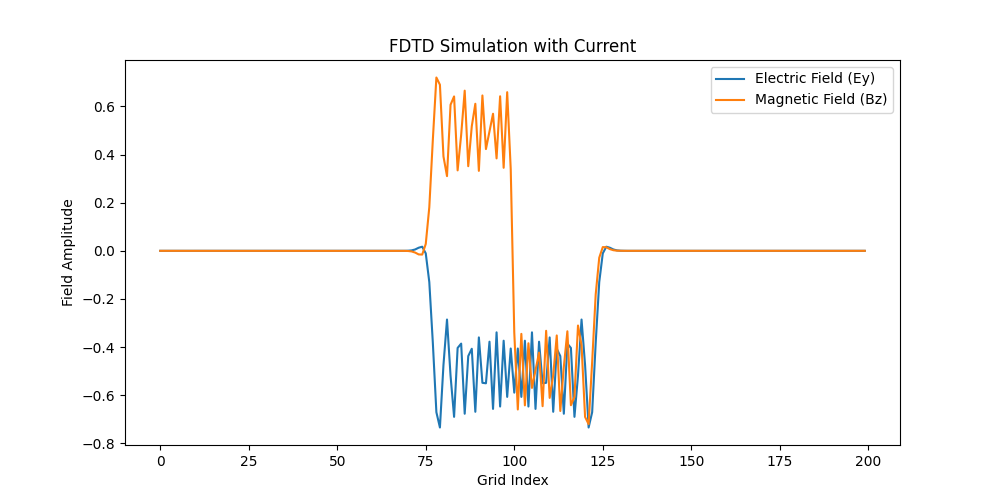
\includegraphics[width=0.8\textwidth]{materials/Figure_50.png}
    \caption{At \( T = 50 \), the fields exhibit more defined wave patterns. The electric field's amplitude starts to increase, demonstrating the effect of periodic boundary conditions that begin to influence the results as the wave reflects back from the boundaries.}
\end{figure}

\subsection{Field Evolution at \( T = 200 \)}
\begin{figure}[H]
    \centering
    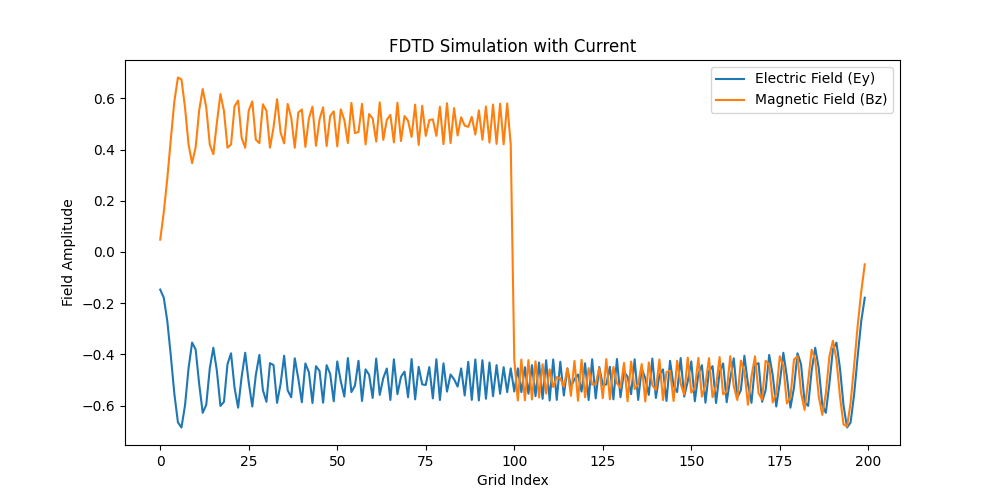
\includegraphics[width=0.8\textwidth]{materials/Figure_200.png}
    \caption{By \( T = 200 \), the influence of the injected current becomes more pronounced, resulting in more significant fluctuations in the magnetic field. This stage shows the electric and magnetic fields interacting dynamically, with visible effects of the current shaping the waveforms across the grid.}
\end{figure}

\section{Conclusion}

In this project, we successfully integrated the effects of a current \( J \) in a 1D FDTD simulation, modeling the interaction between an ion and an electron with opposing velocities at the center of the domain. The simulation results demonstrate how the current affects the electromagnetic fields within the simulation grid. Significant field fluctuations and pattern changes were observed, particularly as the simulation progressed to later time steps. These findings underscore the critical role of current in shaping electromagnetic field dynamics and highlight the effectiveness of the FDTD method in capturing complex wave behaviors in electromagnetics. This project enhanced computational skills in simulating and visualizing physical phenomena.


\section*{References}
\begin{enumerate}
    \item \textbf{Mamanchuk N., University of Tsukuba}, Github, \today. Available online: \url{https://github.com/RIFLE}
    % \item \textbf{Company}, Name of Work, year. Available online: \url{https://...} [Accessed: yyyy-mm-dd]
\end{enumerate}

\end{document}
